\section{Prover Backend and Real Proof Behavior (Stage 5)}
\label{sec:proof_delay_impact}
Stage 5 benchmarks replaced the Mock Prover with the production RISC0 Prover Backend (utilizing Groth16 proof compression) to profile actual cycle scaling, segment boundaries, proving wall-clock times, and on-chain verification gas under controlled conditions.
\begin{figure}[H]
    \centering
    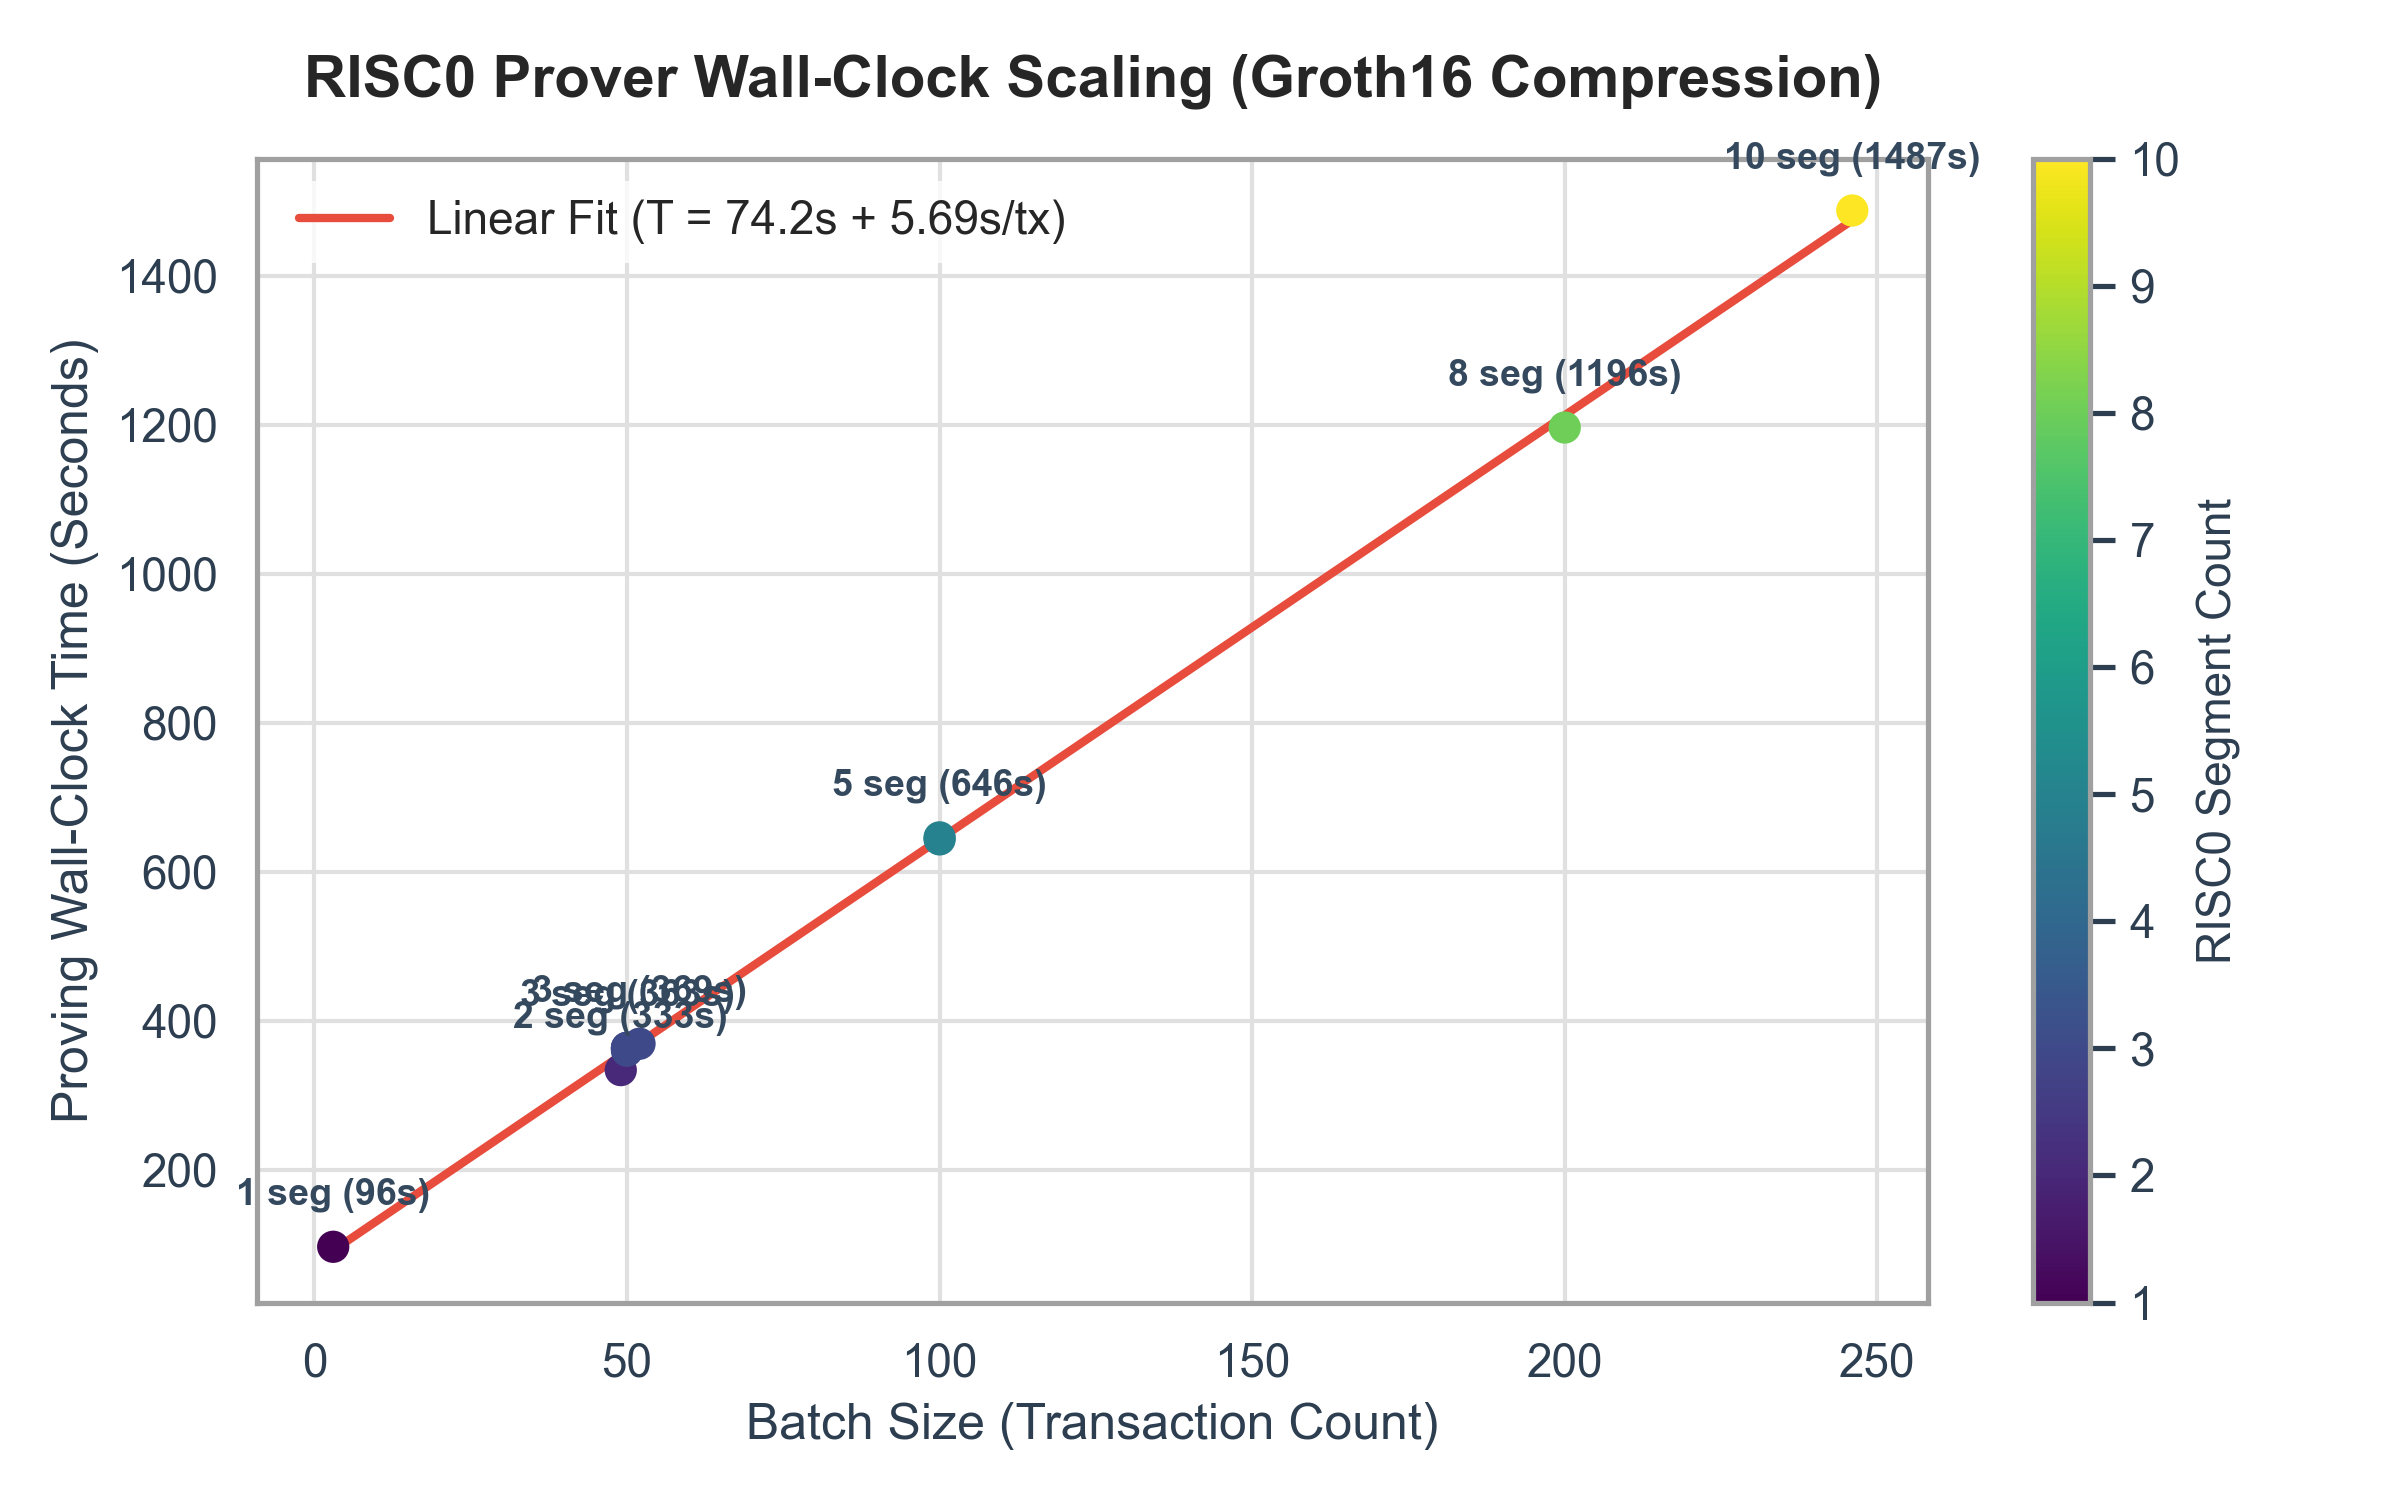
\includegraphics[width=0.90\textwidth]{figures/chapter5/risc0_latency.png}
    \caption{RISC0 zkVM Proving Time (seconds) and Segment Count as a Function of Target Batch Size.}
    \label{fig:risc0_latency}
\end{figure}
\subsection{Prover Wall-Clock Time Amortization}
Zero-knowledge proof generation exhibits a high fixed setup overhead. A linear regression of proving time $T(N)$ as a function of batch size $N$ yields the model:
\begin{equation}
T(N) = A + B \cdot N
\end{equation}
where $A$ represents the fixed compiler loading, setup, and SNARK-wrapping overhead (modeled at \textbf{70 to 80 seconds}), and $B$ represents the marginal proving cost (modeled at \textbf{~5.7 seconds per transaction}).
Because of this fixed cost, small batches represent a highly inefficient use of proving resources. Scaling up the batch size distributes this fixed overhead across a larger transaction pool, reducing the proving wall-clock time per transaction:
\begin{itemize}
    \item \textbf{Batch Size 50 (s5\_real\_bs\_0050):} Amortized proving cost was \textbf{7.5 seconds per transaction}.
    \item \textbf{Batch Size 500 (s5\_real\_bs\_0500):} Amortized proving cost dropped to \textbf{6.0 seconds per transaction}.
\end{itemize}
\subsection{zkVM Cycles and the Segment Step-Function}
Evaluating the zkVM guest logs reveals that each L2 transaction consumes between \textbf{41,000 and 45,000 cycles} depending on the state-access footprint. RISC0 executes and proves guest code in segments of exactly $2^{20} = 1,048,576$ instructions. Because proving is performed segment-by-segment, the wall-clock proving time scales in a step-function governed by segment boundaries, with each additional segment adding approximately \textbf{140 to 150 seconds}:
\begin{itemize}
    \item \textbf{Batch Size 3 (trailing batch):} 262,144 cycles $\rightarrow$ \textbf{1 segment} $\rightarrow$ \textbf{96.2 seconds}.
    \item \textbf{Batch Size 49 (trailing batch):} 2,097,152 cycles $\rightarrow$ \textbf{2 segments} $\rightarrow$ \textbf{333.4 seconds}.
    \item \textbf{Batch Size 50:} 2,162,688 cycles (crosses segment boundary) $\rightarrow$ \textbf{3 segments} $\rightarrow$ \textbf{362.3 seconds}.
    \item \textbf{Batch Size 100:} 4,227,072 cycles $\rightarrow$ \textbf{5 segments} $\rightarrow$ \textbf{645.8 seconds}.
    \item \textbf{Batch Size 200:} 8,388,608 cycles $\rightarrow$ \textbf{8 segments} $\rightarrow$ \textbf{1,196.0 seconds}.
    \item \textbf{Batch Size 246:} 10,485,760 cycles $\rightarrow$ \textbf{10 segments} $\rightarrow$ \textbf{1,487.3 seconds}.
\end{itemize}
This non-linear step-function behavior implies that sequencers should ideally be "cycle-aware," sealing batches right before crossing a segment boundary to optimize proving resource utilization.
\subsection{ZK-Proof Succinctness}
Regardless of the batch size or the number of L2 transactions packaged (from 3 to 246), the final compressed Groth16 proof submitted to L1 was always exactly \textbf{256 bytes}. The verification cost on L1 remains constant, demonstrating the cryptographic succinctness of the modular rollup model.
\subsection{Finalization Time (Hard Finality)}
Batch finalization time (hard finality) is heavily dominated by the proof generation delay. While soft finality (the sequencer sealing and executing the batch locally) is achieved in seconds, hard finality (the submission and verification of the validity proof on L1) requires waiting for the RISC0 prover. In Stage 5, this introduces a finality gap ranging from \textbf{317 seconds} (for a batch of 50 txs) to \textbf{1,487 seconds} (for a batch of 246 txs). This highlights why ZK-rollups must separate the user-facing soft finality from the L1 settlement hard finality.

\subsection{Queue Backpressure}
High proof delays caused backpressure. While the sequencer could continue accepting transactions and forming batches (soft finality), the pipeline downstream (Executor and Submitter) became compute-bound. This highlights the necessity for highly parallelized prover networks in production rollups to prevent the proof-generation stage from completely throttling L1 settlement throughput.
